
\documentclass[journal]{IEEEtran}

\IEEEoverridecommandlockouts                              % This command thanks command
%\overrideIEEEmargins
% See the \addtolength command later in the file to balance the column lengths
% on the last page of the document

%\def\baselinestretch{0.9999}

%\input{boldfacemath}

%\usepackage{exsheets}



% save and then undefine the offending command
% we need \makeatletter because \@undefined uses the special @ character.
\makeatletter
\let\IEEEproof\proof
\let\IEEEendproof\endproof
\let\proof\@undefined
\let\endproof\@undefined
\makeatother

% The following packages can be found on http:\\www.ctan.org
%\usepackage{graphics} % for pdf, bitmapped graphics files
%\usepackage{epsfig} % for xpostscript graphics files
%\usepackage{mathptmx} % assumes new font selection scheme installed
%\usepackage{times} % assumes new font selection scheme installed
\usepackage{amsmath} % assumes amsmath package installed
\usepackage{amssymb}  % assumes amsmath package installed
\usepackage{amsthm}
\usepackage{amsfonts}
\usepackage{mathtools}

% Text
\usepackage{comment}
\usepackage[normalem]{ulem}
%\usepackage[inline]{enumitem}
%let\labelindent\relax % Since the \labelindent command exists for legacy reasons in the IEEE template, you can simply "disable" it by adding the following before importing the enumitem package
%\usepackage{enumitem}
\usepackage{bm}
\providecommand{\bm}{\pmb}

%\usepackage{flushend}

\newtheorem{prop}{Proposition}
\newtheorem{cor}{Corollary}
\newtheorem{defin}{Definition}
\newtheorem{fact}{Fact}
\newtheorem{thm}{Theorem}[section]
\newtheorem{lem}[thm]{Lemma}
\newtheorem*{Zorn}{Zorn’s Lemma}
\theoremstyle{definition}
\newtheorem{dfn}{Definition}
\theoremstyle{remark}
\newtheorem*{rmk}{Remark}
\newtheorem{theorem}{Theorem}[section]
\newtheorem{remark}[theorem]{Remark}

\newtheorem{problem}{Problem}

\usepackage{verbatim}

\usepackage{color}
%\usepackage{subfig}
\usepackage{graphicx}
%\usepackage{caption}
\usepackage{esvect}



%\usepackage{mathptmx}
\usepackage{times}

%%%%%%%%%%%%%%%%%%%%%%%%%%%%%%%%%%%%%%%%%%%%%

\usepackage[ruled,vlined,linesnumbered]{algorithm2e}
%\usepackage[noend]{algorithmic}
\usepackage{algorithmicx}
\usepackage{algpseudocode}

%%%%%%%%%%%%%%%%%%%%%%%%%%%%%%%%%%%%%%%%%%%%%
\graphicspath{{images/}}

\usepackage[us]{datetime}
\usepackage{caption}
\captionsetup{font=small}


%\documentclass[a4, 10pt, conference]{ieeeconf}

 \usepackage[usenames,dvipsnames,table]{xcolor}

\usepackage{hyperref} %pdf with links and toc on the left
\hypersetup{
    colorlinks,
    citecolor=black,
    filecolor=black,
    linkcolor=black,
    urlcolor=black,
    pdfauthor={},
    pdfsubject={},
    pdftitle={}
}

\usepackage{todonotes}
%\usepackage{todonotes} lets you insert notes of stuff to do with the syntax \todo{Add details.}

\usepackage{graphicx}
% \usepackage{graphicx} manage external pictures

\usepackage{latexsym}
\usepackage{color}
% \usepackage{color} adds support for colored text

\usepackage{cite}

% \usepackage{cite} assists in citation management

\usepackage{caption}
%\usepackage{caption} allows customization of appearance and placement of captions for figures, tables, etc.
%\usepackage{subcaption}
\usepackage{subfig}


\usepackage{tikz}
\usepackage{adjustbox}
\usetikzlibrary{shapes,arrows}

% ---------- added packages -----------------------------------
\usepackage{tabularx, booktabs}
\newcolumntype{Y}{>{\centering\arraybackslash}X}
\usepackage{multirow}
\usepackage{paralist}
\usepackage{booktabs}
%\usepackage[table,xcdraw]{xcolor}
% ---------- New Symbols and Commands -------------------------
\usepackage{accents}
% ---------- Standard Commands ------------------

\usepackage{color}
\newcommand\red[1]{{\textcolor{red}{#1}}}
\newcommand\blue[1]{{\textcolor{blue}{#1}}}

\newcommand{\DS}[1]{\red{DS: #1}}
\newcommand{\MANU}[1]{\blue{MANU: #1}}
% ---------- new variables ------------------
\newcommand{\Hinf}{$H_\infty$\xspace}
\newcommand{\photoa}{PH-A}
\newcommand{\photob}{PH-B}
\newcommand{\photodistance}{d}


% ---------- new commands ------------------
\newcommand{\vect}[1]{\bm{#1}}		% vectors
\newcommand{\matr}[1]{\bm{#1}}		% matrices
\newcommand{\nR}[1]{\mathbb{R}^{#1}}		% real number
\newcommand{\nT}[1]{\mathbb{T}^{#1}}		% real number
\newcommand{\define}{:=}			% define symbol
\newcommand{\modulus}[1]{\left| #1 \right|}	% abs
\newcommand{\matrice}[1]{\begin{bmatrix} #1 \end{bmatrix}}	% matrix
\newcommand{\smallmatrice}[1]{\left[\begin{smallmatrix} #1 \end{smallmatrix}\right]}	% matrix
\newcommand{\cosp}[1]{\cos \left( #1 \right)}	% cos with brace
\newcommand{\sinp}[1]{\sin \left( #1 \right)}	% sin with brace
\newcommand{\determinant}[1]{\text{det}\left(#1\right)} 	% determinant
\newcommand{\sgn}[1]{\text{sgn}\left( #1 \right)}			% signum
\newcommand{\atanTwo}[1]{{\rm atan2}\left( #1\right)}		% atan2
\newcommand{\acotTwo}[1]{{\rm acot2}\left( #1\right)}		% acot2
\newcommand{\upperRomannumeral}[1]{\uppercase\expandafter{\romannumeral#1}}	% roman numbers
\newcommand{\lowerromannumeral}[1]{\romannumeral#1\relax}
\newcommand{\vSpace}{\;\,}
\newcommand{\ubar}[1]{\underaccent{\bar}{#1}}

%-----------Functions------------------------
\newcommand{\minEig}[1]{\lambda_{\text{min}}[#1]}
\newcommand{\maxEig}[1]{\lambda_{\text{max}}[#1]}
\newcommand{\transp}{^\top}


% --------- References ----------------------
\newcommand{\fig}{Fig.~}	% figure ref
\newcommand{\eqn}{Eq.~}	% equation ref
\newcommand{\tab}{Tab.~}	% table ref
\newcommand{\cha}{Chap.~}	% chapter ref
\newcommand{\sect}{Sec.~}	% section ref
\newcommand{\alg}{Algorithm~}

% --------- Variables -----------------------

% General
\renewcommand{\frame}{\mathcal{F}}		% frame
\newcommand{\origin}{O}						% origin
\newcommand{\vX}{\vect{x}}					% x-axis
\newcommand{\vY}{\vect{y}}					% y-axis
\newcommand{\vZ}{\vect{z}}					% z-axis
\newcommand{\pos}{\vect{p}}				% position vector
\newcommand{\dpos}{\vect{v}}				% velocity vector
\newcommand{\rotMat}{\matr{R}}				% rotation matrix
\newcommand{\rotMatVectAngle}[2]{\rotMat_{#1}(#2)}	% rotation matrix representing the rotation about a vector of a certain angle
\newcommand{\vZero}{\vect{0}}				% vect/matr of zeros
\newcommand{\en}[1]{\vect{e}_{#1}}		% vect e_n
\newcommand{\eye}[1]{\matr{I}_{#1}}
\newcommand{\zeros}[1]{\matr{0}_{#1}}
\newcommand{\skewmatr}[1]{\big[{#1}\big]_\times}
\newcommand{\skewmatrS}[1]{\matr{S}({#1})}

% World frame
\newcommand{\frameW}{\frame_W}			% world frame
\newcommand{\originW}{\origin_W}		% origin world frame
\newcommand{\xW}{\vX_W}				% x-axis world frame
\newcommand{\yW}{\vY_W}				% y-axis world frame
\newcommand{\zW}{\vZ_W}				% z-axis world frame
\newcommand{\dxW}{\dot{\vX}_W}

% Background
\newcommand{\samplingPeriod}{T_s}
\newcommand{\samplingFrequency}{f_s}
\newcommand{\vwater}{\bar{v}_{water}}
\newcommand{\vhex}{\bar{v}_{hex}}
\newcommand{\vfluid}{\bar{v}_{fl}}
\newcommand{\samplesWater}{N_{water}}
\newcommand{\samplesHex}{N_{hex}}
\newcommand{\samplesfl}{N_{fl}}
\newcommand{\samplesflk}{N_{fl,k}}
\newcommand{\samples}{n}
\newcommand{\avgL}[1]{L_{#1}}
\newcommand{\vnominal}{v_{n}}
\newcommand{\channelArea}{A}
\newcommand{\slugvelocity}{v_{sl}}


% Modeling 2nd Order Systems
\newcommand{\settlingtime}{t_s}
\newcommand{\naturalfrequency}{w_n}
\newcommand{\damping}{\xi}
\newcommand{\bias}{b_{0}}

% Modeling
\newcommand{\eigenvalues}[1]{\lambda_{#1}}
\newcommand{\slugfrequencyerror}{e_{\slugfrequency}}

% Flow rates
\newcommand{\flowratecommand}{F^{\star}_{fl}}
\newcommand{\flowrate}{F}
\newcommand{\flowratewatercommand}{F^{\star}_{water}}
\newcommand{\flowratehexcommand}{F^{\star}_{hex}}
\newcommand{\urate}{u_{fl}}
\newcommand{\uratess}{\expectedflowrate}
\newcommand{\urateinit}{u_{fl_{0}}}

\newcommand{\uratecommand}{\urate^{\star}}
\newcommand{\uratecommandwater}{u^{\star}_{water}}
\newcommand{\uratecommandhex}{u^{\star}_{hex}}
\newcommand{\out}{y}


% Frequency
\newcommand{\slugfrequency}{f_{sl}}
\newcommand{\slugfrequencyinit}{f_{sl_{0}}}
\newcommand{\slugfrequencyss}{\tilde{f}_{sl}} %steady-state
\newcommand{\currentslugfrequency}{f_{sl}^c}
\newcommand{\desiredslugfrequency}{f_{sl}^d}
\newcommand{\slugfrequencyDes}{\desiredslugfrequency} %easy to use command wrt desiredsslugfrequency. This is the reason of the repetition.

% Control
\newcommand{\samplesk}{k}
\newcommand{\modelgain}{K_p}
\newcommand{\predictionHorizon}{N_p}
\newcommand{\controlHorizon}{N_c}
\newcommand{\controlVector}{\Delta \matr{U}}
\newcommand{\controlvector}[1]{\Delta \uratecommand({#1})}
\newcommand{\controlsample}{\uratecommand}
\newcommand{\referenceVector}{\matr{R}_{\slugfrequency}}
\newcommand{\outputVector}{\matr{Y}}
\newcommand{\outputvector}[1]{y_{fl}(#1)}
\newcommand{\costfunction}{\matr{J}}
\newcommand{\performanceMatrix}{\bar{\matr{R}}}
\newcommand{\slugfrequencymean}{\mu_{\slugfrequency}}
\newcommand{\slugfrequencystd}{\sigma_{\slugfrequency}}
\newcommand{\expectedflowrate}{\tilde{u}_{fl}}

\newcommand{\transitionMatrix}{\matr{F}}
\newcommand{\controlMatrix}{\matr{\Phi}}
\newcommand{\state}{x} 
\newcommand{\timeWindow}{t_w}


%My symbols
\newcommand{\abscissa}{x}
\newcommand{\ordinate}{y}
\newcommand{\mean}[1]{<V_{#1}(t)>}
\newcommand{\meann}{<V(t)>}
\newcommand{\spatialmean}[3]{V_{#1}({#2},{#3},t)}
\newcommand{\width}{W_{ROI}}
\newcommand{\height}{H_{ROI}}
\newcommand{\frequency}{f_i}
\newcommand{\amplitude}{A}
\newcommand{\range}{Range<V_x(t)>}
\newcommand{\peak}{AP}
\newcommand{\particles}{<N_p(t)>}

%Measurement units
\newcommand{\pixel}{pixels}
\newcommand{\apixel}{pixel}
\newcommand{\density}{Kg/m^3}
\newcommand{\hertz}{Hz}
\newcommand{\flow}{ml/min}
\newcommand{\seconds}{s}
\newcommand{\framerate}{FPS}
\DeclarePairedDelimiter{\norm}{\lVert}{\rVert} % norm

\captionsetup[subfigure]{labelformat=simple, labelsep=colon}
\makeatletter
\renewcommand*{\thesubfigure}{(\alph{subfigure})} 
\makeatother
%\makeatother
\pagestyle{headings}

%%%%%%%%%%%%%%%%%%%%%%%%%%%%%%%%%%%%%%%%%%%%%%%%%%%%%%%%%%%%%%%%%%%%%%%%%%%%%%%

\title{DPIV Analysis and Real Time Implementation}


\author{E. Cutuli${^{1}}$, G. Stella${^{1}}$, D. Sanalitro${^{1}}$, M. Bucolo${^{1}}$~\IEEEmembership{Senior Member,~IEEE}

\thanks{$^1$Department of Electrical Electronic and Computer Science Engineering, University of Catania, CT, Italy. {\tt \scriptsize\href{mailto:uni391076@studium.unict.it}{\mbox{uni391076@studium.unict.it}}
\scriptsize\href{mailto:emaunuela.cutuli@phd.unict.it}{\mbox{emanuela.cutuli@phd.unict.it}}
\scriptsize\href{mailto:giovanna.stella@phd.unict.it}{\mbox{giovanna.stella@phd.unict.it}}
\scriptsize\href{mailto:dario.sanalitro@unict.it}{\mbox{dario.sanalitro@unict.it}}}. 
\scriptsize\href{mailto:maide.bucolo@unict.it}{\mbox{maide.bucolo@unict.it}}}. 
}

%\thanks{Digital Object Idenitifier (DOI): see top of this page}




%%%%%%%%%%%%%%%%%%%%%%%%%%%%%%%%%%%%%%%%%%%%%%%%%%%%%%%%%%%%%%%%%%%%%%
\begin{document}
%%%%%%%%%%%%%%%%%%%%%%%%%%%%%%%%%%%%%%%%%%%%%%%%%%%%%%%%%%%%%%%%%%%%%%


\maketitle

%%%%%%%%%%%%%%%%%%%%%%%%%%%%%%%%%%%%%%%%%%%%%%%%%%%%%%%%%%%%%%%%%%%%%%
\begin{abstract}

\end{abstract}
%%%%%%%%%%%%%%%%%%%%%%%%%%%%%%%%%%%%%%%%%%%%%%%%%%%%%%%%%%%%%%%%%%%%%%

\begin{IEEEkeywords}
	Signal processing, Micro-optofluidic device, Data-driven Modelling
\end{IEEEkeywords}

\section{Introduction}

This paper ecc...

\subsection{Paper main contributions}


\section{Materials and Methods}

\subsection{System Design and Hardware Platform Realization}\label{sec:design}

\begin{figure}[!h]
	\centering
	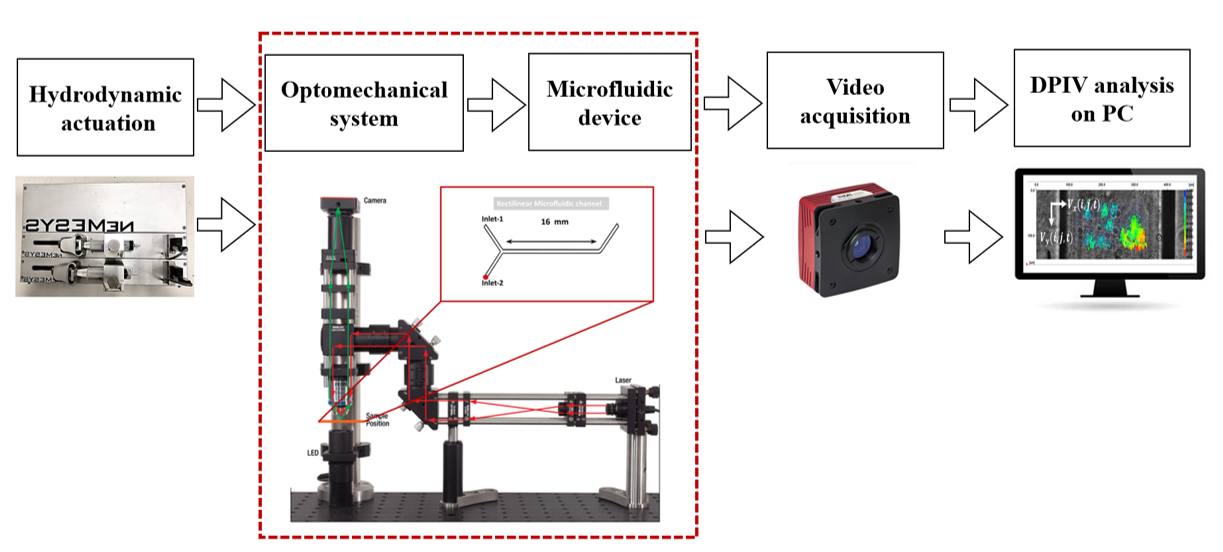
\includegraphics[width=1\columnwidth]{images/PlatformDesign}
	\centering{\caption{\label{Platform}System Design and Hardware Platform Realization block schemes }}
\end{figure}

From a methodological point of view, the experimental characterization of the process takes place through the acquisition of videos that allow studying different interaction mechanisms between particles/cells subjected to different external stresses.
The captured videos are then analyzed using Digital Particle Image Velocimetry (DPIV).
In order to study the different interaction mechanisms between particles in micro-channels subject to external hydrodynamic actuation, the system is composed of i) the hydrodynamic actuation system, ii) the optomechanical system, iii) the microfluidic device,, iv) a video-acquisition system, v)  a PC where the algorithm runs, as shown in \fig\ref{Platform}.

%$\flowrate$, $\flowratewatercommand$,$\channelArea$ are all examples of variables defined in "symbol-definition.tex"

\subsection{DPIV Online Platform Implementation}\label{sec:method}

\DS{Provide a little bit of scientific context where DPIV has been used. I would try to make a small search if a part from this work~\cite{2017-CaiSanBucOrtCabInt}, offline/online versions have been presented.  }
In this paper, a DPIV online platform implementation for data acquisition and processing is proposed. Starting from a pre-existing DPIV platform that works offline, a new version of the same algorithm
that works online has been implemented. ~\fig\ref{Algorithms} shows a schematic of the two implementations. The feature that most diversifies the two algorithms is based on the fact that the offline algorithm works on a video acquired in a moment before the analysis that is carried out and through a different software from the one on which the analysis routine runs.



\begin{figure}[t]
	\centering
	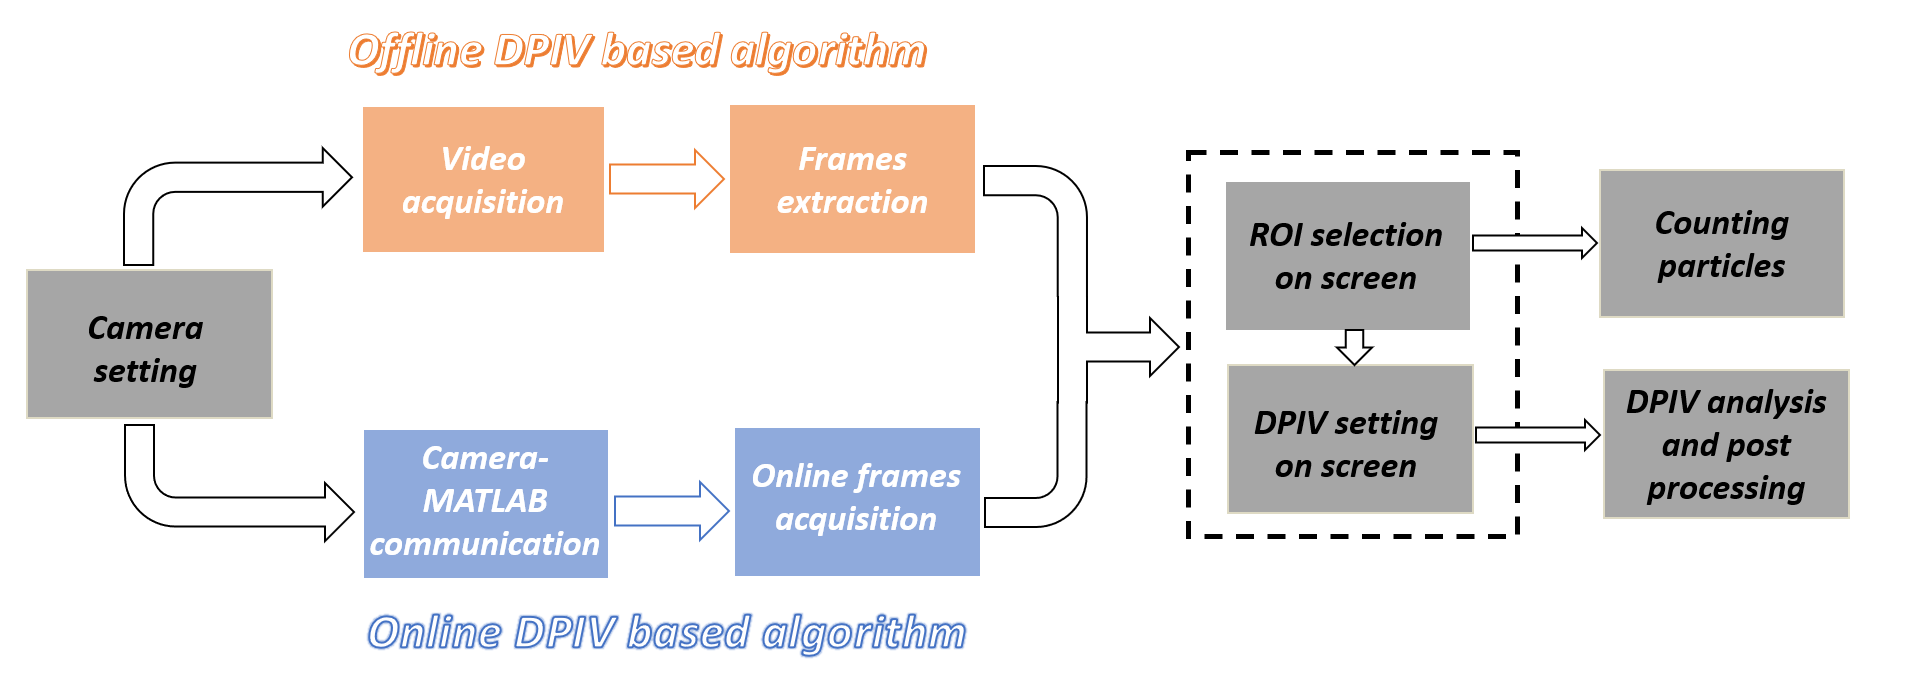
\includegraphics[width=1\columnwidth]{images/Algorithms}
	\centering{\caption{\label{Algorithms}Online algorithm implementation }}
\end{figure}

\begin{figure}[t]
	\centering
	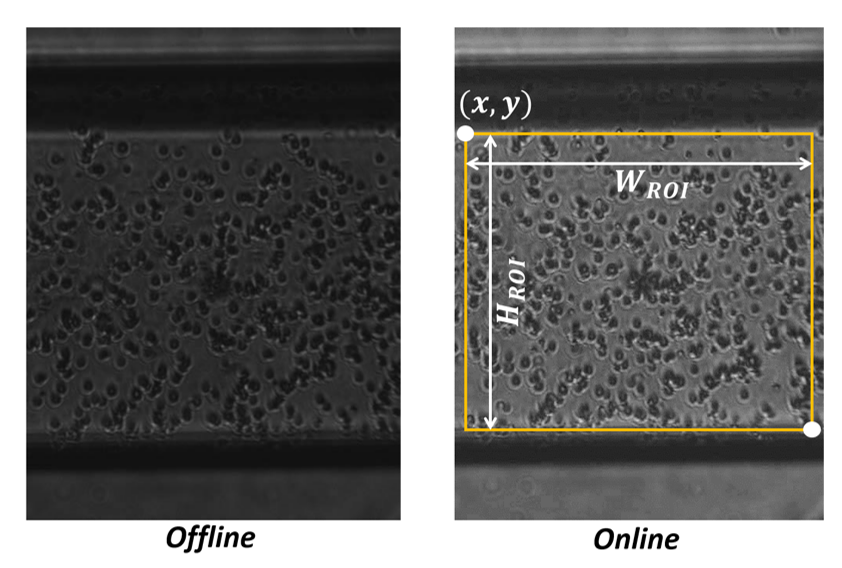
\includegraphics[width=0.8\columnwidth]{images/frames}
	\centering{\caption{\label{frame} Offline and Online frame in comparison with the same camera parameters. Region of Interest (ROI) coordinates selection in the Online frame. }}
\end{figure}

The first step, common to both platforms, involves the camera parameters setting, through the following quantities: i) pixelsize obtained from the camera datasheet, ii) magnification based on the optical equipment used in the experimental setup, iii) exposure time chosen on the basis of experimental needs, iv) image gain chosen on the basis of experimental needs. 
The major contribution of the Online version is represented by the acquisition that takes place in an online mode through the communication between the CCD camera and MATLAB downloading the \textbf{Windows SDK and Doc. for Scientific Cameras}. This allows to capture process frames directly from the MATLAB routine and they are ready to be used for the analysis. The Offline version, on the other hand, provides for a further step of uploading on MATLAB the video previously acquired through a dedicated software and unpack it into the corresponding frames. 
Online frames acquisition through MATLAB allows to obtain a higher resolution process frame for the same camera parameters as it is shown in ~\fig\ref{frame}.
\\Having the data available, the algorithm proceeds in a similar way in the two platforms.
\\An on-screen ROI selection procedure has been introduced by setting the left-top corner of the image as the starting pixel and the right-down corner of the image as the end pixel. The resulting coordinates for the selection of the ROI are represented in ~\fig\ref{frame}: the abscissa ($x$) and ordinate ($y$) of the left-top point and the width ($W_{ROI}$) and height ($H_{ROI}$) of the region itself, obtained from the selection of the right-down point.
\\A DPIV analysis followed by a micro-particles counting procedure are at this point carried out for the predefined interrogation Regions of Interest (ROIs). A DPIV-based algorithm provides instantaneous velocity measurements and visualization. The DPIV approach \DS{When something is not a contribution of the paper, we will add a reference} consists of a first collection of the time-varying velocity vector maps through the evaluation of the cross-correlation between ROIs of consecutive pairs of images. The velocity spatial distribution along the horizontal $V_x(i,j,t)$ and vertical $V_y(i,j,t)$ directions is obtained for each pairs of frame. Spatial averaging is done so that a single velocity value is obtained for each map. By repeating this procedure for all the frames, two signals representing the trends of the average speed over time are given, respectively $<V_x(t)>$ and $<V_y(t)>$.
The preliminary step of DPIV setting concerns the possibility of opting to a multi-pass discrete Fourier transform (DFT) for the DPIV analysis, through the following parameters i) number of passes that could be chosen from 1 to 4, ii) step size, iii) interrogation areas varying with the first parameter. 
A multi-pass DFT in frequency domain, as implemtend by the PIVlab tool, could be used in order to increase the accuracy. In this experimental campaign the analysis was conducted by a three-passes DFT, reaching a good compromise between the resolution and the computational time. The three interrogation areas in pixels were chosen as follows: $Area1=64$, $Area2=32$ and $Area3=16$. The step size was set equal to the half of the last interrogation area ($Area3=16$), resulting in a value equal to 8 pixels.
\\There is a further choice of performing the analysis in the whole ROI (single section) or by dividing the ROI into three horizontal sections, parallel to the particles' motion direction (three sections) for a deeper investigation. This choice allows to highlight through the results the different particles' average speed in the edges of the channel, which is lower than the one at the center of the channel.
Despite this possibility, in this experimental campaign it was chosen to conduct the analysis only in the single section because the goal was to compare the behavior of different types of particles and not to compare the same cells in different portions of the ROI.
\\The second type of analysis that this platform provides is the micro-particles counting. This procedure is based on highlighting the particles in the image distinguishing them from the background. It provides a continuous counting in the time of the micro-particles number in the investigated area, avoiding any manual and individual selecting of the frames to be studied. It analyzes the video frame by frame, counts the number of particles and collects this information in a signal.
 \\The following steps for the counting operation are all based on image processing:
 
 \begin{enumerate}
 	\item ROI selection;
 	\item Conversion to greyscale;
 	\item Duplication of the image;
 	\item Application of a gaussian filter (radius equal to 5);
 	\item Difference between the original image and the duplicated one;
 	\item Binarization of the image;
 \end{enumerate}
At this point a function takes as input the binary image. It traces the exterior boundaries of particles and gives the number of them found.
Important parameters to be set are the minimum and maximum dimensions of the searched object in pixels, in order to count among the found micro-particles only those that have an appropriate size. For the yeast cells and the silica beads the minimum area was set to 1 pixel and the maximum was set to 2 pixels. There is another parameter to be set based on the shape of the object that is a threshold value chosen to define the circularity. Due to the circular geometry of the micro-particles, the threshold was set equal to 1 that indicates a perfect circle.
Having defined all the parameters, the exterior boundaries of micro-particles are traced and the number of them is found for each frame.

\subsection{Experimental Setup and Campaigns}

The experimental set-up is composed of a syringe pump, a microfluidic chip, an opto-mechanical system and a personal computer. A representation of it is reported in ~\fig\ref{setup}. Syringe pumps (neMESYS low-pressure module, Cetoni GmbH,
Korbussen, Germany) were used to inject the sample of particles or cells suspended in a fluid in the Y-junction squared rectilinear micro-channel (SMS0104, Thinxxs, Zweibrucken, Germany), 16~$[\rm mm]$ long and with a diameter of 320~$[\rm~\mu m]$ (see ~\fig\ref{Platform}).


A CCD camera (340M Fast Frame, Thorlabs, Newton, NJ, USA) with a resolution of $640x480$ pixels (pixel size of 7.4~$[\rm~\mu m]$, square) was included in the optomechanical system ((OTKB/M) Modular Optical Tweezers, Thorlabs, Newton, NJ, USA). Visible light from the LED source illuminates the sample and is then imaged
on the CCD camera.
The CCD camera was connected through a USB connection with a PC for the data acquisition and the subsequent analysis phase in the dedicated software platform.


\begin{figure}[t]
	\centering
	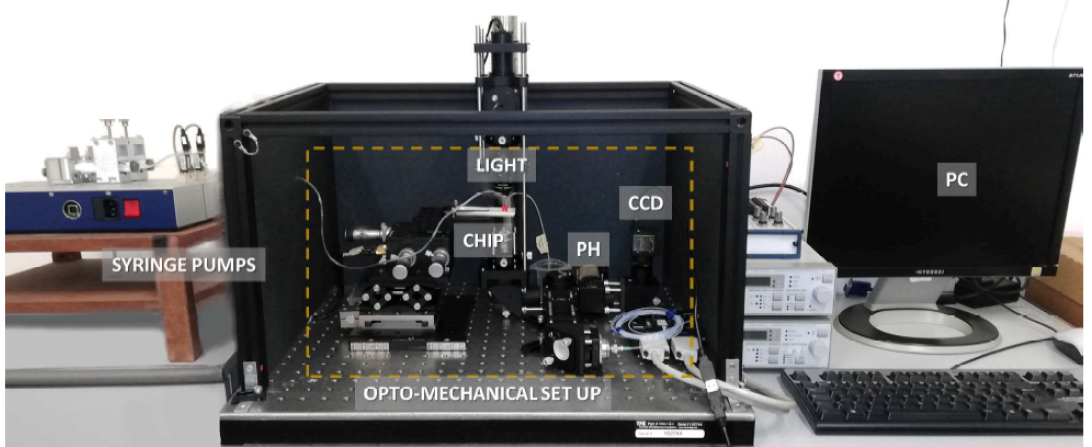
\includegraphics[width=1\columnwidth]{images/setup}
	\centering{\caption{\label{setup}A picture showing the experimental set-up.}}
\end{figure}

A magnification of 10X (PLN, Olympus, Tokyo, Japan) has been used to scale up the channel images to be able to see more detail and increasing resolution.
Acquisitions and analyzes were performed using a SAMSUNG Galaxy Book PC, with an Intel Core i7 processor, INTEL Iris Xe Graphics, 16 GB RAM and 512 GB SSD.
\\The fluids employed for the experiments were obtained by diluting micro-particles in different solutions. The micro-particles were of two types: cells of eukaryotic origins with a diameter of 5~$[\rm~\mu m]$ and artificial silica beads with a diameter of 6~$[\rm~\mu m]$. Two types of particles have been used to investigate and compare the different behaviors of cells and synthetic particles. Their physical properties, such as mass, radius, volume and density, are summerized in ~\tab\ref{properties}. Four different types of yeast cell living conditions have been examined. In particular viable cells, 2 days overgrowth, 5 days overgrowth and exposed to cell death stimuli with hydrogen peroxide ($H_2O_2$). 
Yeast cells were diluted in a saline solution, the phospate buffered saline (PBS, density of 1072 $Kg/m^3$). By contrast, Silica beads micro-particles were diluted in two different solutions. A first one (density of 1200 $Kg/m^3$) obtained by combining 20\% of water with 80\% of glycerol to avoid the deposition of the particles at the bottom of the channel thanks to the increment of the fluid density. The second solution is represented by PBS.
The microfluidic chip was fed with fluid on which an oscillating flow was imposed.
At the beginning a PBS flow and then a glycerol-water flow, without micro-particles suspendend on it, was recorded to quantify the effect of the fluid backgroung in the images. It was injected through syringe pumps with an external oscillating pressure at a frequency of $f_i= 0.1 Hz$ and an amplitude of $A=0.1 ml/min$. 
\\The other 40 experiments that have been carried out are summarized in ~\tab\ref{offlineexp} and ~\tab\ref{onlineexp}, distinguished according to the software platform used to analyze them (Offline or Online). Experiments with viable yeast cells and beads in glycerol-water solution were performed twice, to compare the results obtained with the two different platforms and test their consistency.
For all categories of cells and particles, the sample of fluid was fed into the micro-channel using an oscillating flow at a fixed frequency of $f_i= 0.1 Hz$ and five different amplitude values $A \in{0.05, 0.07, 0.1, 0.15, 0.2 ml/min}$.


% Please add the following required packages to your document preamble:
% \usepackage{booktabs}
\begin{table}[t]
	\begin{tabular}{@{}lcccc@{}}
		\toprule
		\multicolumn{1}{c}{\textbf{Micro-particles}} & \textbf{\begin{tabular}[c]{@{}c@{}}Mass\\ {[}$Kg${]}\end{tabular}} & \textbf{\begin{tabular}[c]{@{}c@{}}Radius\\ {[}$m${]}\end{tabular}} & \textbf{\begin{tabular}[c]{@{}c@{}}Volume\\ {[}$m^3${]}\end{tabular}} & \textbf{\begin{tabular}[c]{@{}c@{}}Density\\ {[}$Kg/m^3${]}\end{tabular}} \\ \midrule
		\textit{Yeast cells}                         & 7.37 e\textasciicircum{}-14                                      & 2.5 e\textasciicircum{}-6                                         & 6.54 e\textasciicircum{}-17                                                          & 1126                                                                                     \\
		\textit{Silica beads}                        & 1.36 e\textasciicircum{}-13                                      & 3.0 e\textasciicircum{}-6                                         & 1.13 e\textasciicircum{}-16                                                          & 1200                                                                                     \\ \bottomrule
	\end{tabular}
\centering{\caption{\label{properties}Physical properties of micro-particles.}}
\end{table}


\begin{table}[t]
	\begin{tabular}{@{}lp{0.85cm}c@{}}
		\toprule
		\rowcolor[HTML]{FFFFFF} 
		\textbf{Micro-particles}                            & \textbf{\begin{tabular}[c]{@{}c@{}}Frequency \\ $f_i$ {[}$Hz${]}\end{tabular}} & \textbf{\begin{tabular}[c]{@{}c@{}}Amplitude \\ $A$\,{[}\,$ml/min${]}\end{tabular}} \\ \midrule
		\textit{Viable Yeast cells}                        & 0.1                                                                       & 0.05, 0.07, 0.1, 015, 0.2                                                                                               \\
		\textit{Yeast cells 2 days overgrowth}             & 0.1                                                                       & 0.05, 0.07, 0.1, 015, 0.2                                                                                               \\
		\textit{Yeast cells 5 days overgrowth}             & 0.1                                                                       & 0.05, 0.07, 0.1, 015, 0.2                                                                                               \\
		\textit{Yeast cells exposed to cell death stimuli} & 0.1                                                                       & 0.05, 0.07, 0.1, 015, 0.2                                                                                               \\
		\textit{Beads in PBS}                              & 0.1                                                                       & 0.05, 0.07, 0.1, 015, 0.2                                                                                               \\
		\textit{Beads in glycerol-water}                   & 0.1                                                                       & 0.05, 0.07, 0.1, 015, 0.2                                                                                               \\ \bottomrule
	\end{tabular}
\centering{\caption{\label{offlineexp}Offline experimetal campaign.}}
\end{table}

\begin{table}[t]
	\begin{tabular}{@{}lcc@{}}
		\toprule
		\rowcolor[HTML]{FFFFFF} 
		\textbf{Micro-particles}          & \textbf{\begin{tabular}[c]{@{}c@{}}Frequency \\ $f_i$ {[}$Hz${]}\end{tabular}} & \textbf{\begin{tabular}[c]{@{}c@{}}Amplitude \\ $A$\,{[}\,$ml/min${]}\end{tabular}} \\ \midrule
		\textit{Viable Yeast cells}    
		     & 0.1                                                                       & 0.05, 0.07, 0.1, 015, 0.2                                                   \\
		\textit{Beads in glycerol-water} & 0.1                                                                       & 0.05, 0.07, 0.1, 015, 0.2                                                   \\ \bottomrule
	\end{tabular}
\centering{\caption{\label{onlineexp}Online experimetal campaign.}}
\end{table}

For each experiment, the sample flow was acquired through a video. The data were recorded considering different time intervals in the two types of algorithms:
\begin{itemize}
	\item \textbf{Offline algorithm}: data recorded for 60 seconds, with a video frame rate of 57 frames per second, around 3420 frames per experiment.
	\item \textbf{Online algorithm}: data recorded for 15 seconds, with a video frame rate of 57 frames per second, around 855 frames per experiment. 
\end{itemize}

% Please add the following required packages to your document preamble:
% \usepackage{booktabs}
\begin{table}[t]
	\begin{tabular}{@{}llc@{}}
		\toprule
		\textbf{}                       & \multicolumn{1}{c}{\textbf{Offline}} & \textbf{Online}                            \\ \midrule
		\textbf{Camera sampling frequency}          & \multicolumn{2}{c}{57 FPS}                                                 \\
		\textbf{Process transient time}             & \multicolumn{2}{c}{2 minutes}                                              \\
		\textbf{Acquisition time window}            & 60 seconds                           & 15 seconds                          \\
		\textbf{DPIV processing time}               & 67 minutes                           & 19 minutes                          \\
		\textbf{Counting particles processing time} & 5 minutes                            & \textit{work in progress}           \\ \bottomrule
	\end{tabular}
\centering{\caption{\label{timing}Experimetal campaign timing.}}
\end{table}

\begin{table}[t]
	\begin{tabular}{@{}llll@{}}
		\toprule
		\textbf{Pixelsize}         & \textbf{Magnification}  & \textbf{Exposure Time}       & \textbf{Image Gain}     \\ \midrule
		\multicolumn{1}{c}{7.4~$[\rm~\mu m]$} & \multicolumn{1}{c}{10X} & \multicolumn{1}{c}{17000~$[\rm~\mu s]$} & \multicolumn{1}{c}{200} \\ \bottomrule
	\end{tabular}
	\centering{\caption{\label{campar}Camera setting parameters. }}
\end{table}

Through some tests, optimal camera parameters were obtained and set equal for all the experiments. In particular, the image gain was set equal to 200 and the exposure time equal to 17000~$[\rm~\mu s]$, resulting in a framerate of 57 FPS. The pixelsize value set at 7.4~$[\rm~\mu m]$ was obtained from the camera datasheet. All camera setting parameters are summerized in ~\tab\ref{campar}.
Another important step to perform before the start of the DPIV and
counting particles analysis is the selection of the ROI.
It was determined as described in \sect\ref{sec:method} and the coordinates are reported in ~\tab\ref{roi} . 

% Please add the following required packages to your document preamble:
% \usepackage{booktabs}
\begin{table}[t]
	\begin{tabular}{@{}lcccc@{}}
		\toprule
		\multicolumn{5}{c}{\textbf{Region of Interest (ROI)}}                                                                                         \\ \midrule
		& \textbf{$x$} & \textbf{$y$} & \textbf{$H_{ROI}$} & \textbf{$W_{ROI}$} \\
		\textit{Yeast cells}  & 6          & 131        & 473                                          & 360                                          \\
		\textit{Silica beads} & 7          & 67         & 467                                          & 411                                          \\ \bottomrule
	\end{tabular}
	\centering{\caption{\label{roi}Region of Interest (ROI) coordinates set for the image area acquired and analyzed in the performed experiments. }}
\end{table}



~\tab\ref{timing} summurized the temporal references that characterized the experimental campaign. They are listed in terms of camera sampling frequency, process transient time, acquisition time window, DPIV and counting particles processing Time. 
\\The values of the processing times depend on the performance of the PC and also on the size of the selected ROI: greater regions of analysis correspond to greater processing times.


\section{Results and discussion}

\subsection{Particles suspended in fluids with different densities}



\subsection{Viable cells, Dead cells and Synthetic Particles in comparison}

\subsection{Online vs Offline}

\section{Conclusions}


\bibliographystyle{IEEEtran}
% DO NOT ERASE THE NEXT LINE,
% ONLY COMMENT IT AND DECOMMENT THE NEXT-NEXT, IF YOU NEED
%\bibliography{./bibCustom}



\end{document}

